% use the MIT thesis document class
\documentclass[12pt]{mitthesis}

% some packages needed for library-compliant typesetting
\usepackage{lgrind}
\usepackage{cmap}
\usepackage[T1]{fontenc}
\pagestyle{plain}

% packages I put into the template 
\usepackage{pdfpages} % to include pdfs
\usepackage{caption} % for caption*
\usepackage{graphicx}
\usepackage{chapterbib} % for bibliographies in each chapter
\usepackage{tocloft} % for fixing table of contents
\usepackage[linktocpage=true]{hyperref} % for internal links
\usepackage{booktabs} % for nice tables
\usepackage{lscape} % for a landscape page (extra-wide table)

% options for controlling the table of contents typesetting
\setcounter{tocdepth}{0} % only show chapters in table of contents
\renewcommand{\cftchapfont}{\rmfamily} % chapters in not bold
\renewcommand{\cftchappagefont}{\rmfamily} % page in not bold

% for inputting the ancient Greek
\usepackage[utf8x]{inputenx}
\usepackage[polutonikogreek,english]{babel}
\usepackage{epigraph}

\begin{document}

\title{Quantitative modeling for microbial ecology and clinical trials}

\author{Scott Wilder Olesen}
\prevdegrees{B.A., Williams College (2010) \\
    M.A.St., University of Cambridge (2011) \\
    M.Phil., University of Cambridge (2012)}
\department{Department of Biological Engineering}

\degree{Doctor of Philosophy in Biological Engineering}

% Valid degree months are September, 
% February, or June.  The default is June.
\degreemonth{September}
\degreeyear{2016}
\thesisdate{19 August 2016}

%% By default, the thesis will be copyrighted to MIT.  If you need to copyright
%% the thesis to yourself, just specify the `vi' documentclass option.  If for
%% some reason you want to exactly specify the copyright notice text, you can
%% use the \copyrightnoticetext command.  
%\copyrightnoticetext{\copyright IBM, 1990.  Do not open till Xmas.}

% If there is more than one supervisor, use the \supervisor command
% once for each.
\supervisor{Eric J. Alm}{Professor}

% This is the department committee chairman, not the thesis committee
% chairman.  You should replace this with your Department's Committee
% Chairman.
\chairman{Forest White}{Chair of Graduate Program, Department of Biological Engineering}

% Make the titlepage based on the above information.  If you need
% something special and can't use the standard form, you can specify
% the exact text of the titlepage yourself.  Put it in a titlepage
% environment and leave blank lines where you want vertical space.
% The spaces will be adjusted to fill the entire page.  The dotted
% lines for the signatures are made with the \signature command.
\maketitle

% The abstractpage environment sets up everything on the page except
% the text itself.  The title and other header material are put at the
% top of the page, and the supervisors are listed at the bottom.  A
% new page is begun both before and after.  Of course, an abstract may
% be more than one page itself.  If you need more control over the
% format of the page, you can use the abstract environment, which puts
% the word "Abstract" at the beginning and single spaces its text.

% You can either \input (*not* \include) your abstract file, or you can put
% the text of the abstract directly between the \begin{abstractpage} and
% \end{abstractpage} commands.
\cleardoublepage
\setcounter{savepage}{\thepage}
\begin{abstractpage}
%% The text of your abstract and nothing else (other than comments) goes here.
%% It will be single-spaced and the rest of the text that is supposed to go on
%% the abstract page will be generated by the abstractpage environment.
Microbial ecology has benefited from the decreased cost and increased quality
of next-generation DNA sequencing. In general, studies that use DNA sequencing
are no longer limited by the sequencing itself but instead by the acquisition
of the samples and by methods for analyzing and interpreting the resulting
sequence data.
In this thesis, I describe the results of three projects that address challenges
to interpreting or acquiring sequence data.
In the first project,
I developed a method for analyzing the dynamics of the relative abundance of
operational taxonomic units measured by next-generation amplicon sequencing in 
microbial ecology experiments without replication. In the second project, I
and my co-author combined a taxonomic survey of a dimictic lake, an ecosystem-level
biogeochemical model of microbial metabolisms in the lake, and the results of
a single-cell genetic assay to infer the identity of taxonomically-diverse,
putatively-syntrophic microbial
consortia. In the third project, I and my co-author developed a model of differences
in the efficacy that stool from different donors has when treating patients
via fecal microbiota transplant. We use that model to compute statistical
powers and to optimize clinical trial designs.
Aside from contributing scientific conclusions about each system, these
methods will also serve as a conceptual framework for future efforts to address
challenges to the interpretation or acquisition of microbial ecology data. 

\end{abstractpage}

\cleardoublepage

\section*{Acknowledgments}

Many people contributed to my PhD, including:
\begin{itemize}
    \item my advisor Eric Alm, whom I thanks for for his mentorship,
    unswerving advocacy, and delightful collegiality,
    \item my thesis committee members Paul Blainey and Martin Polz,
    \item my scientific mentors Pierre Wiltzius, Sophia Gershman, Daniel Aalberts, 
        Dieter Bingemann, Sarah Bolton, Ward Lopes, Paul Selvin, and David Wales,
    \item my collaborators and mentors inside the Alm Lab, especially Sarah Preheim,
        Ilana Brito, Thomas Gurry, Sarah Spencer, and Su Vora,
    \item my outside collaborators, especially Terry Hazen and his group,
    \item Doug Lauffenburger and Forest White for making Biological Engineering a
        great community to live and work in,
    \item my colleagues and friends in the Alm Lab,
    \item my colleagues and friends at MIT, especially the 2012 class of
        Biological Engineering graduate students, Jaime Goldstein, and the founding class
        of Writing Lab Fellows,
    \item my parents Mary and Neil and my brother Andrew.
\end{itemize}
My PhD was also aided by funding from Williams College's Dr. Herchel Smith
Fellowship, MIT's Presidential Fellowship, the National Science Foundation's
Graduate Research Fellowship, BP, and the Department of Energy.

\pagestyle{plain}
%% This file simply contains the commands that actually generate the table of
%% contents and lists of figures and tables.  You can omit any or all of
%% these files by simply taking out the appropriate command.
\begingroup
\raggedright
\tableofcontents
\endgroup

\newpage
%\listoffigures
%\newpage
%\listoftables


% include each tex file
%% This is an example first chapter.  You should put chapter/appendix that you
%% write into a separate file, and add a line \include{yourfilename} to
%% main.tex, where `yourfilename.tex' is the name of the chapter/appendix file.
%% You can process specific files by typing their names in at the 
%% \files=
%% prompt when you run the file main.tex through LaTeX.
\chapter{Introduction}

Microbes, the oldest and most diverse type of life on Earth, are essential to
human life and industry. Microbes catalyze key biogeochemical cycles, clean up
toxic pollution, and can prevent or cure disease. Microbial ecology---the study of
microbes' relationships with one another and their environment---has
benefited tremendously from nucleic acid sequencing technology. RNA was first
sequenced in the 1960s~\cite{sanger_two_1965}. Microbiologists, notably Carl
Woese, used sequences of 16S rRNA, present in all bacteria and archaea, to
develop a more accurate ``tree'' of microbial
life~\cite{woese_phylogenetic_1977,pace_phylogeny_2012}. DNA was first
sequenced in the 1970s, and 16S rRNA gene sequences were directly amplified
from the environment and sequenced for the first time in
1990~\cite{giovannoni_genetic_1990,case_use_2007}. High-throughput sequencing
and sample multiplexing~\cite{hamady_error_2008} have enabled microbial
ecologists to collect large datasets at a decreasing cost of time and money.

Even as tools to process nucleic acid sequence data for microbial ecology
mature, there remain challenges to interpreting sequence data and integrating
them with other types of microbial ecology data. In this thesis, I present
the results of three projects that aim, in part, to help interpret microbial
sequence data. In Chapter 2, I discuss the Treatment Effect eXplorer for
Microbial Ecology Experiments (\texttt{texmex}), an analytical tool designed to
extract information about the dynamics of microbial taxa from microbial
ecology experiments with few timepoints and few or no replicates. In Chapter 3,
I discuss a novel biogeochemical model of a lake ecosystem, a novel
network-analysis method for organizing microbial ecology sequence data,
and intepretative frameworks for linking those models and methods with
survey data and a single-cell genetic assay. In Chapter 4, I discuss an
``omics-free'' model designed to guide the design and execution of clinical
trials that use fecal microbiota transplants. In the rest of this chapter,
I introduce and contextualize these contributions; in the final chapter,
I discuss the limitations and potential extensions of theses studies.

\section{Interpreting microbial ecology sequence data}
A major challenge in analyzing and interpreting microbial ecology experiments
that use sequencing is to determine which microbial taxa are meaningfully
different in abundance. Most approaches to this question are statistical and
focus, one-by-one, on the abundances of each taxon, analogous to methods that
identify differentially expressed genes in transcriptomic data (e.g.,
DESeq~\cite{anders_high_2010}). The $t$-test and simple ordinations have been
mainstays of this type of analysis for microbial ecology sequence
data~\cite{segata_metagenomic_2011}.

This approach presents difficulties when there are few or no biological
replicates, compositional effects affect measurements of composition, or when
it is important to integrate pre-test samples. I therefore developed
\texttt{texmex}, which considers the distribution of abundances of microbial taxa
\emph{within} a sample to make a more coherent comparison of abundances across
samples. I noted that microbial abudances within a sample follow the Poisson
lognormal distribution, which had been previously studied in macroecology, and
used that distribution to ``normalize'' the abundances of microbial taxa
within samples before comparing abundances across samples. As described in
Chapter 2, I applied this technique to short timeseries experiments measuring
the response of ocean microbial communities to amendment with crude oil,
verifying the presence of known oil degraders and suggesting that other
organisms, implicated in other crude oil microcosm experiments, are also
involved in crude oil degradation.

Microbial ecology surveys that use taxonomic marker gene sequence data
confront a different problem: the relationship between phylogeny and
function. Taxonomic marker gene sequencing (e.g., 16S rRNA amplicon sequencing)
provides information about microbial community structure but provides
only indirect information about microbial community function~\cite{langille_predictive_2013}. Metagenomic
sequencing provides more direct information about community function,
but it is expensive and mostly discards information about the relationships
between phylogeny and function.

In Chapter 3, I describe a set of tools used to identify potential consortia
of cooperating organisms in a natural ecosystem. This study includes a
taxonomic survey of the environment, an ecosystem-level model of microbial
metabolisms, and a single-cell genetic assay that links phylogeny and
function. For that study, I developed a network-analysis method (operational
ecological units) for the survey data and an interpretative framework
(inferred biomass) for the model result. These tools provided a conceptual
link between all three types of data, which were together essential for
the putative \textit{in situ}, perturbation-free identification of
microbial consortia.

\section{Clinical trial design}
Fecal microbiota transplantation (FMT) is a highly effective intervention for
patients suffering from recurrent \textit{Clostridium difficile}, a
common nosocomial infection~\cite{kassam_fecal_2013}. As the gut microbiome is
assigned an increasingly important role in the development and maintenance of host
gut health, immunity, and even psychology, the success of FMT for \textit{C.
difficile} has generated interest in using FMT to treat other conditions to
which an ``unhealthy'' gut microbiota may
contribute~\cite{smits_therapeutic_2013}. Although the exact mechanism by which FMT
treats \textit{C. difficile} is not well understood, a few clinical
trials have already experimented with using FMT as a treatment for other
conditions, and many more trials for a variety of diseases will probably begin
in the coming years.

These early trials using FMT to treat conditions beyond \textit{C. difficile}
have had some confusing and disappointing results. Of two recent
trials using FMT to treat inflammatory bowel disease, one
failed~\cite{rossen_findings_2015} and the other produced an unexpected
result: five of six stool donors in the trial appeared to produce results no
better than treating the patients with placebo, while the sixth donor produced
stool that appeared to have substantially greater efficacy~\cite{moayyedi_fecal_2015}.

If this sort of difference in efficacy between donors' stool is real, then
what are the implications for clinical trial design? 
To answer this question, I designed a model of differences in stool
efficacy and used the model to predict the statistical power of typical trial
designs. These results, laid out in Chapter 4, show that, if the results
from this recent inflammatory bowel disease trial are representative, then
FMT's efficacy is only likely to be discovered using larger patient cohorts
and response-adaptive allocation of donors' stool. I used this model
to aid the design of a two-stage phase I clinical trial using FMT to treat
a gastrointestinal condition, and I expect that these power calculations and
adaptive allocation strategies will improve clinical trial design, improving
the probability that patients will have access to a new therapy.

\begin{singlespace}
\bibliography{main}
\bibliographystyle{unsrt}
\end{singlespace}

%% This is an example first chapter.  You should put chapter/appendix that you
%% write into a separate file, and add a line \include{yourfilename} to
%% main.tex, where `yourfilename.tex' is the name of the chapter/appendix file.
%% You can process specific files by typing their names in at the 
%% \files=
%% prompt when you run the file main.tex through LaTeX.
\chapter{A novel analysis method for paired-sample microbial ecology experiments}

The contents of this chapter were published as: 
Olesen SW, Vora S, Techtmann SM, Fortney JL, Bastidas-Oyanedel JR, Rodr\'{i}guez J,
\textit{et al.} (2016) A Novel Analysis Method for Paired-Sample Microbial Ecology
Experiments. \textit{PLoS ONE} \textbf{11}(5): e0154804. doi:10.1371/journal.pone.0154804.

The figures, tables, and supplementary figures and tables are at the end of the chapter.

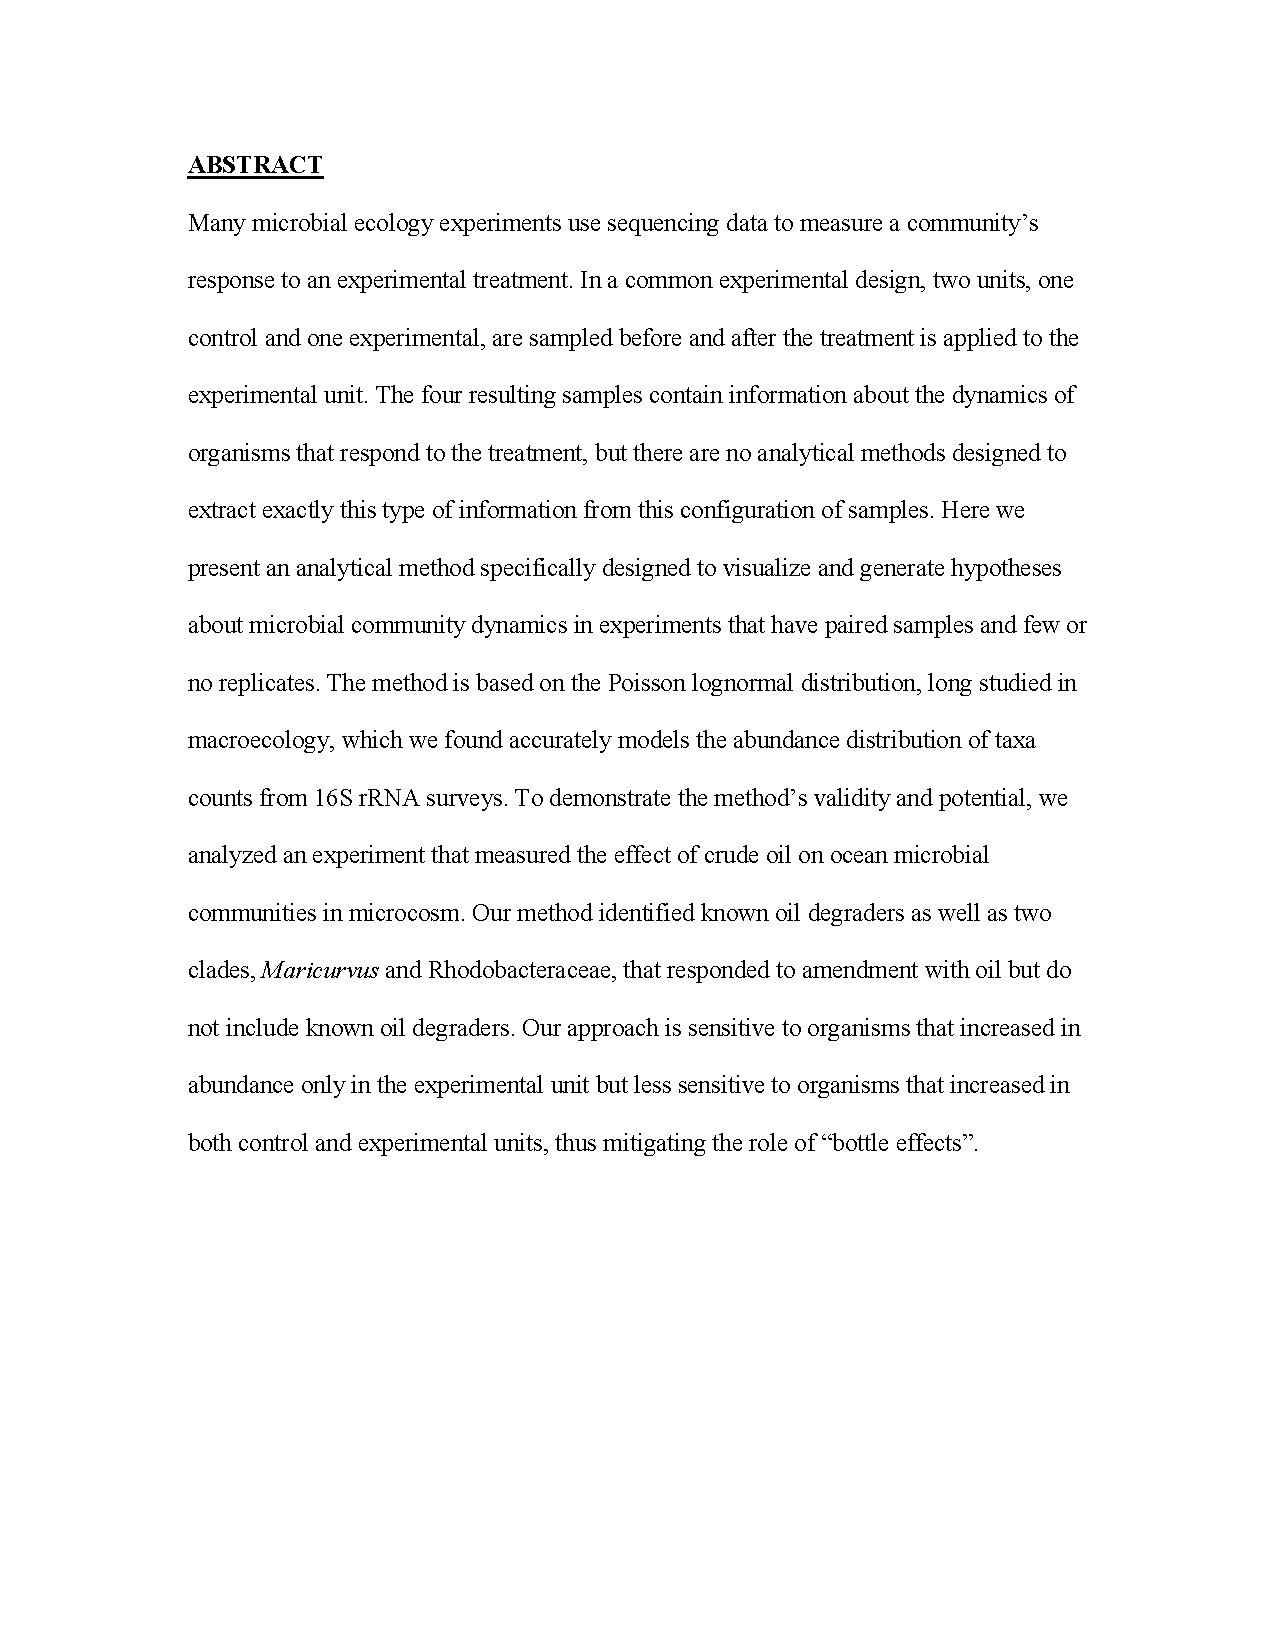
\includepdf[pages=-, pagecommand={\thispagestyle{plain}}, scale=1.0]{texmex/ms}

\clearpage
\begin{figure}[ht]
\centering
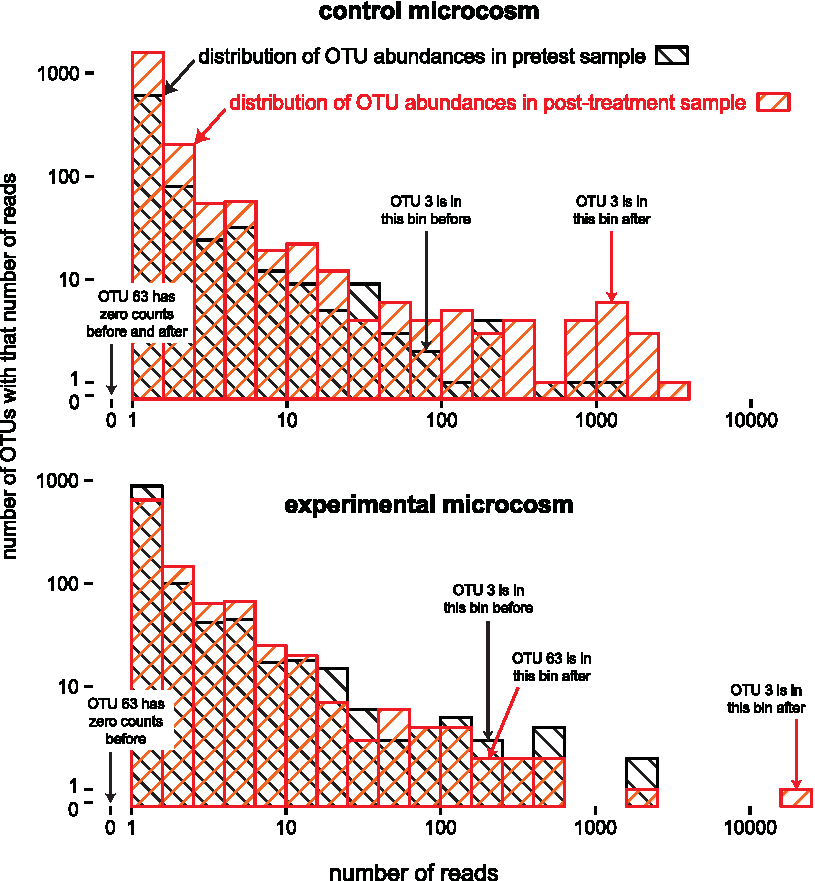
\includegraphics{texmex/fig/fig_1}
\caption*{{\bf Figure 1. OTU dynamics and possible bottle effects in a paired-sample experiment.} 
Four histograms are shown, one each for each sample in the experiment:
control-before (above, black), control-after (above, red), experimental-before
(below, black), experimental-after (below, red). Each histogram shows how many
OTUs (logarithmic $y$-axes) have what number of associated reads (logarithmic
$x$-axis). No bin is shown for OTUs with zero counts. The dynamics of two OTUs
are shown: black arrows point to the abundance bin for OTUs in the ``before''
sample and red arrows point their abundance bins in the ``after'' samples.}
\end{figure}

\clearpage
\begin{figure}[ht]
\centering
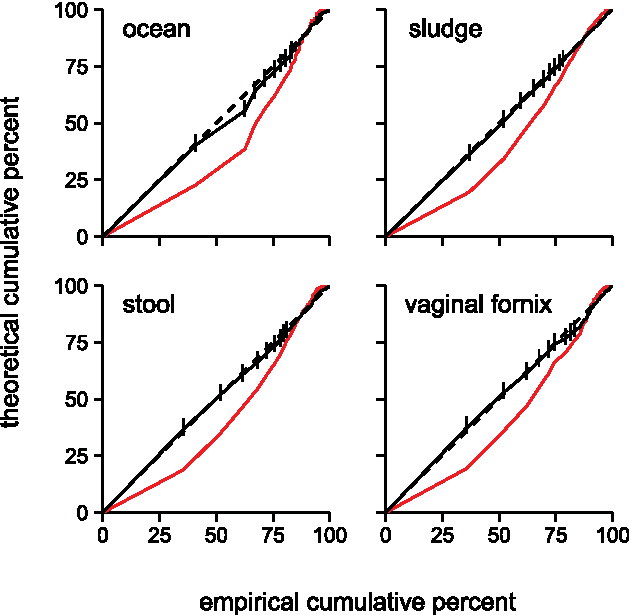
\includegraphics{texmex/fig/fig_2}
\caption*{{\bf Figure 2. TPL distribution fits OTU abundance distributions in multiple ecosystems.}
Probability-probability plots comparing the empirical cumulative distribution
function (horizontal axis) with the theoretical cumulative probability of a TPL
distribution fit to each data set (vertical axis, black solid line). The first
ten data points are marked with vertical dashes: the first dash (furthest lower
left) represents the fraction of OTUs that have 1 read, the second dash
represents the fraction of OTUs with 2 or fewer reads, and so forth. The dotted
black line indicates a perfect fit of the TPL to the empirical distribution ($y = x$).
The theoretical cumulative probability of a simple lognormal distribution
(red line) is shown to emphasize the quality of the TPL fit. The ecosystems are
ocean water from this study (top left), wastewater sludge from this study (top
right), human stool (bottom left; Human Microbiome Project [HMP] sample), and
human vagina (bottom right; HMP sample). 99\% \textit{de novo} OTUs are shown for all
samples.}
\end{figure}

\clearpage
\begin{figure}[ht]
\centering
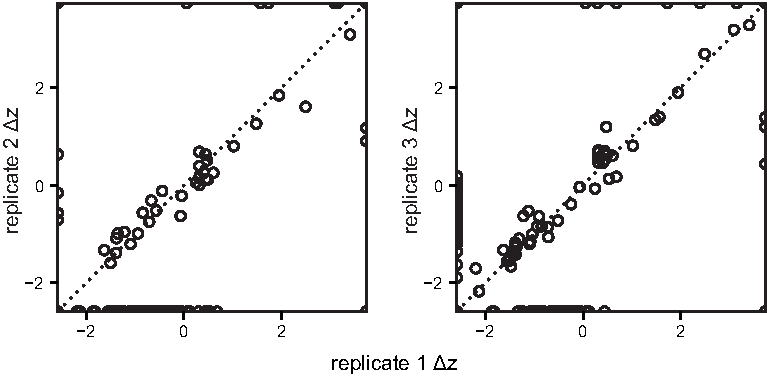
\includegraphics{texmex/fig/fig_3}
\caption*{{\bf Figure 3. OTUs in replicate units have correlated dynamics.}
The dynamics of OTUs (circles) in three replicate bioreactors (replicate 1,
$x$-axis; replicates 2 and 3, $y$-axes) inoculated with the same material and
subjected to the same conditions. The dotted line ($y=x$) indicates a perfect
correlation: an OTU on this line would have exactly the same $\Delta z$ in both
replicates, while deviations show differences in dynamics. For example, in the
left plot, OTUs above the dotted line experienced a greater increase in
abundance in replicate 2 than in replicate 1 (or, a smaller decrease in 2 than
in 1), while OTUs below the line ``grew more'' in replicate 2 than in replicate 1
(or, ``died less'' in 2 than in 1). OTUs with infinite $\Delta z$ are plotted on the
plot's borders (e.g., the points in the lower-right corner of the first plot
represent OTUs that have $\Delta z = +\infty$ in replicate 1 and $\Delta z = -\infty$ in replicate 2).}
\end{figure}

\clearpage
\begin{figure}
\centering
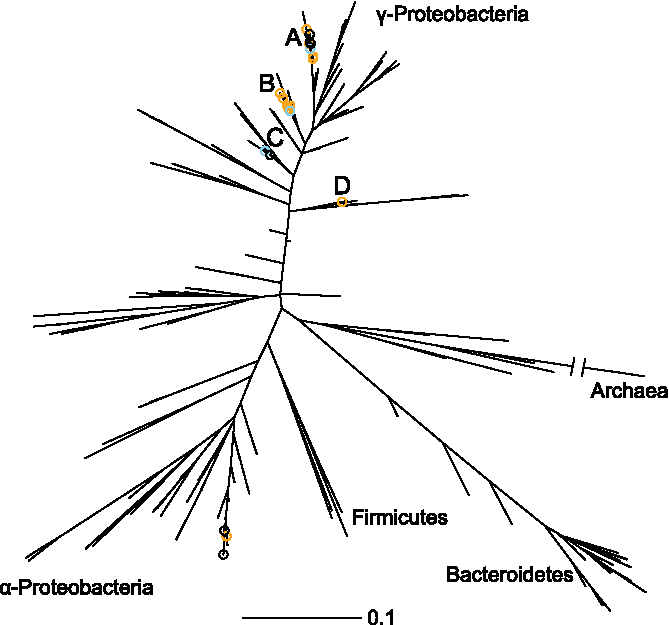
\includegraphics{texmex/fig/fig_4}
\caption*{{\bf Figure 4. OTUs that respond to oil appear in five clades.}
On a phylogenetic tree built from the 16S sequences, organisms potentially
responding to crude oil are marked with open circles. OTUs that satisfy the $\Delta z$
criteria are marked with blue circles, OTUs that satisfy the $\Delta F$ criteria are
marked with orange circles, and OTUs that satisfy both are marked with black
circles. Information about the taxonomy and dynamics of these sequences are
shown in Table 1. The five clades (A through E) are labeled, and select
taxonomic groups are labeled to help orient the reader. The Archaea branch is
truncated. Scale bar: substitutions per site.}
\end{figure}

\clearpage
\begin{table}
\caption*{{\bf Table 1. OTUs with dynamic behavior in response to amendment with oil}
(\textit{on next page}).
All OTUs that satisfied the $\Delta z$ or $\Delta F$ criteria are listed. The first
three columns show taxonomy. The most specific RDP taxonomic
classification with at least 80\% bootstrap support is shown. The next
two columns indicate whether the OTU satisfied the $\Delta z$ criteria, the $\Delta F$
criteria, or both. The next six columns show the changes in relative
abundance ($\Delta \mathrm{r.a.}$), rescaled reads $z$, and cumulative distribution
function $F$ in the control (``ct'') and experimental (``ex'') units. The
value $\Delta z = \mathrm{n.a.}$ is shown for OTUs that had zero counts at both
timepoints in that microcosm; $\Delta z = \infty$ is shown for OTUs had zero counts
before the treatment and more than zero counts after the treatment.}
\end{table}

\clearpage
\begin{landscape}
\begin{table}
\centering
\begin{tabular}{*{12}{l}}
\toprule
 &  &  & \multicolumn{2}{c}{criteria} & \multicolumn{2}{c}{$\Delta\mathrm{r.a.}$} & \multicolumn{2}{c}{$\Delta z$} & \multicolumn{2}{c}{$\Delta F$} &  \\
\cmidrule(r){4-5} \cmidrule(r){6-7} \cmidrule(r){8-9} \cmidrule(r){10-11}
Clade & Classification & support & $\Delta z$ & $\Delta F$ & ct & ex & ct & ex & ct & ex & OTU ID \\
\midrule
A & \textit{Maricurvus} & 0.95 & * &  & 0.033 & 0.739 & 1.382 & 1.419 & $-0.0002$ & 0.0041 & 3 \\
 & \textit{Maricurvus} & 0.87 &  & * & 0 & 0.008 & n.d. & $\infty$ & 0 & 0.9958 & 63 \\
 & $\gamma$-Proteobacteria & 1 &  & * & 0 & 0.0033 & n.d. & $\infty$ & 0 & 0.9942 & 107 \\
 & \textit{Maricurvus} & 0.87 &  & * & 0 & 0.003 & n.d. & $\infty$ & 0 & 0.9939 & 111 \\
 & \textit{Maricurvus} & 0.96 & * & * & 0 & 0.0013 & 0.827 & $\infty$ & 0.1429 & 0.9883 & 119 \\
 & \textit{Maricurvus} & 0.97 & * &  & $-0.0002$ & 0.0002 & 0.115 & $\infty$ & 0.0263 & 0.9292 & 256 \\
 & \textit{Maricurvus} & 0.9 & * &  & $-0.0001$ & 0.0005 & 0.402 & $\infty$ & 0.1649 & 0.9659 & 262 \\
 & \textit{Maricurvus} & 0.94 &  & * & 0 & 0.0007 & n.d. & $\infty$ & 0 & 0.9767 & 291 \\
B & \textit{Pseudomonas} & 1 & * &  & 0.0027 & 0.0629 & 1.137 & 1.073 & 0.014 & 0.0063 & 14 \\
 & \textit{Pseudomonas} & 0.99 &  & * & 0 & 0.0142 & n.d. & $\infty$ & 0 & 0.9961 & 42 \\
 & \textit{Pseudomonas} & 0.91 &  & * & 0 & 0.0112 & n.d. & $\infty$ & 0 & 0.996 & 53 \\
 & Pseudomonaceae & 0.82 &  & * & 0 & 0.0045 & n.d. & $\infty$ & 0 & 0.995 & 88 \\
 & \textit{Pseudomonas} & 0.99 &  & * & 0 & 0.0025 & n.d. & $\infty$ & 0 & 0.9931 & 120 \\
 & \textit{Pseudomonas} & 0.91 &  & * & 0 & 0.0018 & n.d. & $\infty$ & 0 & 0.9913 & 167 \\
 & \textit{Pseudomonas} & 1 &  & * & 0 & 0.0016 & n.d. & $\infty$ & 0 & 0.9903 & 174 \\
C & \textit{Alcanivorax} & 1 & * & * & $-0.0001$ & 0.0004 & 0.402 & $\infty$ & 0.1649 & 0.9599 & 206 \\
 & \textit{Alcanivorax} & 1 & * &  & $-0.0007$ & $-0.0001$ & 0.007 & $-0.143$ & $-0.0143$ & 0.0148 & 270 \\
D & \textit{Methylophaga} & 1 &  & * & 0 & 0.0006 & n.d. & $\infty$ & 0 & 0.9739 & 210 \\
E & Rhodobacteraceae & 1 & * & * & $-0.0003$ & 0.0008 & $-0.167$ & $\infty$ & $-0.1188$ & 0.9799 & 104 \\
 & Rhodobacteraceae & 1 & * & * & 0.0003 & 0.0003 & 1.237 & $\infty$ & 0.2935 & 0.9384 & 105 \\
 & Rhodobacteraceae & 1 & * & * & $-0.0002$ & 0.0001 & 0.115 & $\infty$ & 0.0263 & 0.7678 & 226 \\
 & Rhodobacteraceae & 1 &  & * & 0 & 0 & n.d. & $\infty$ & 0 & 0.6098 & 288 \\
\bottomrule
\end{tabular}
\end{table}
\end{landscape}

\clearpage
\begin{figure}[ht]
\centering
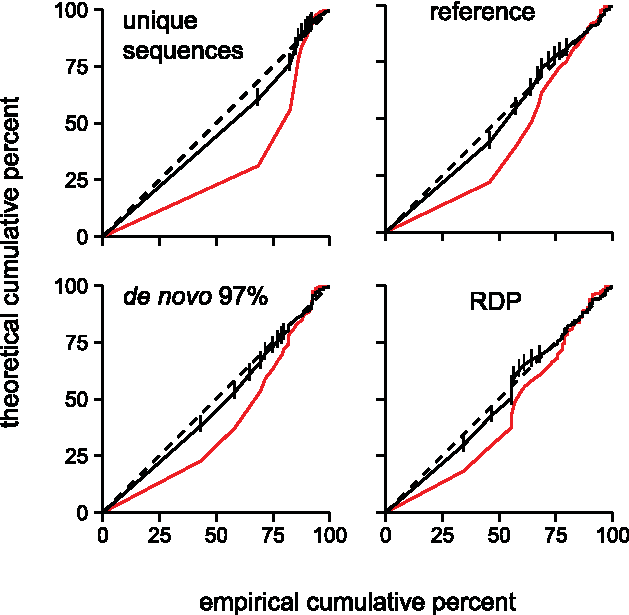
\includegraphics{texmex/fig/fig_s1}
\caption*{{\bf S1 Fig. TPL fits OTUs called by different methods.}
Probability-probability plots
comparing the empirical cumulative distribution function ($x$-axis) with the
theoretical cumulative probability of a TPL distribution fit to the
distribution of OTUs computed using different OTU-calling methods ($y$-axis,
black line). This is same ocean sample as in Figures 1 and 2. The first ten
data points are marked with vertical dashes: the first dash (furthest lower
left) represents fraction of OTUs with 1 read, the second dash represents the
fraction of OTUs with 2 or fewer reads, and so forth. The dotted black line
indicates a perfect fit ($y = x$). The theoretical cumulative probability of a
simple lognormal distribution fit to each OTU distribution (red) is shown to
emphasize the quality of the TPL fit. The methods are unique sequences (i.e.,
100\% identity OTUs; top left), 97\% reference-based OTUs from Greengenes (top
right), \textit{de novo} 97\% OTUs (bottom left), and genus-level OTUs computed with RDP
(bottom right). The empirical goodness-of-fit test described in the main text
yields $p = 0.35, 0.40, 0.44, 0.41$ for these data.}
\end{figure}

\clearpage
\begin{figure}[ht]
\centering
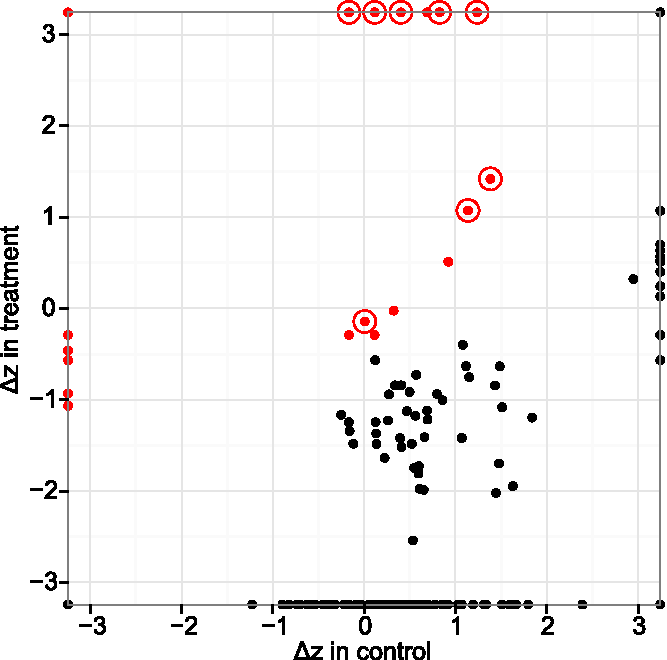
\includegraphics{texmex/fig/fig_s2}
\caption*{{\bf S2 Fig. OTU dynamics measured by $\Delta z$.}
Each OTU present in the microcosm experiment described in the main text is
shown. OTUs that meet the $\Delta z$ criterion described in the text ($\Delta z$ in treatment >
$\Delta z$ in control $- 0.5$) are in red. OTUs that meet the criterion and are among
the 304 most abundant sequences in the four microcosm experiments (i.e., those
shown as blue dots in Figure 4) are circled. OTUs with an undefined $\Delta z$ value in
either microcosm are not shown, while OTUs with infinite $\Delta z$ values are shown at
the border of the figure (e.g., an OTU with $\Delta z = +\infty$ in the control unit and $-\infty$
in the experimental unit would be shown in the lower-left corner).}
\end{figure}

\clearpage
\begin{figure}[ht]
\centering
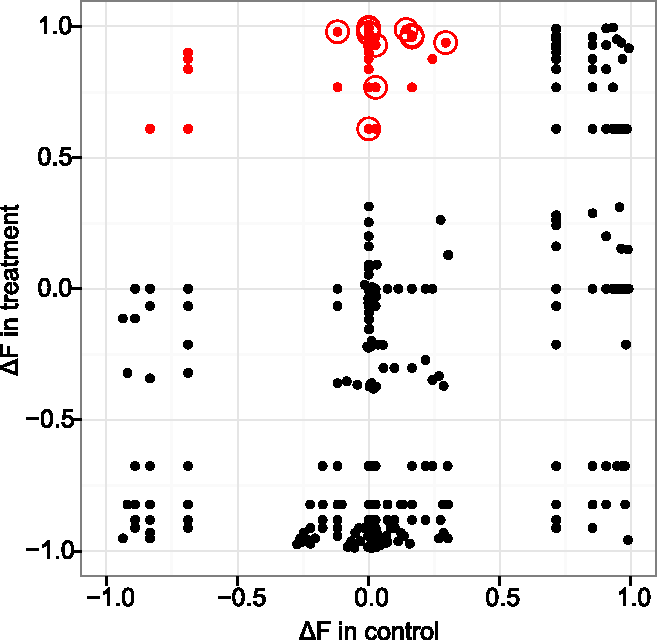
\includegraphics{texmex/fig/fig_s3}
\caption*{{\bf S3 Fig. OTU dynamics measured by $\Delta F$.}
Each OTU present in the microcosm experiment described in the main text is
shown. OTUs that meet the $\Delta F$ criteria described in the text ($\Delta F$ in treatment >
0.5; $\Delta F$ in control $< 0.5$) are in red. OTUs that meet those criteria and are
among the 304 most abundant sequences in the four microcosm experiments (i.e.,
those shown as red dots in Figure 4) are circled.}
\end{figure}

%% This is an example first chapter.  You should put chapter/appendix that you
%% write into a separate file, and add a line \include{yourfilename} to
%% main.tex, where `yourfilename.tex' is the name of the chapter/appendix file.
%% You can process specific files by typing their names in at the 
%% \files=
%% prompt when you run the file main.tex through LaTeX.
\chapter{Surveys, simulation, and single-cell assays relate function and phylogeny in a lake ecosystem}
\label{ch:lake}

The contents of this chapter were accepted as: 
Sarah P. Preheim$^*$, Scott W. Olesen$^*$ (these authors contributed equally), Sarah J. Spencer, Arne Materna,
Charuleka Varadharajan, Matthew Blackburn, Jonathan Friedman, Jorge
Rodr\'{i}guez, Harold Hemond and Eric J. Alm.
(2016) \textit{Nature Microbiology}.

The figures are at the end of the chapter. The Supplementary Information is in Appendix A.

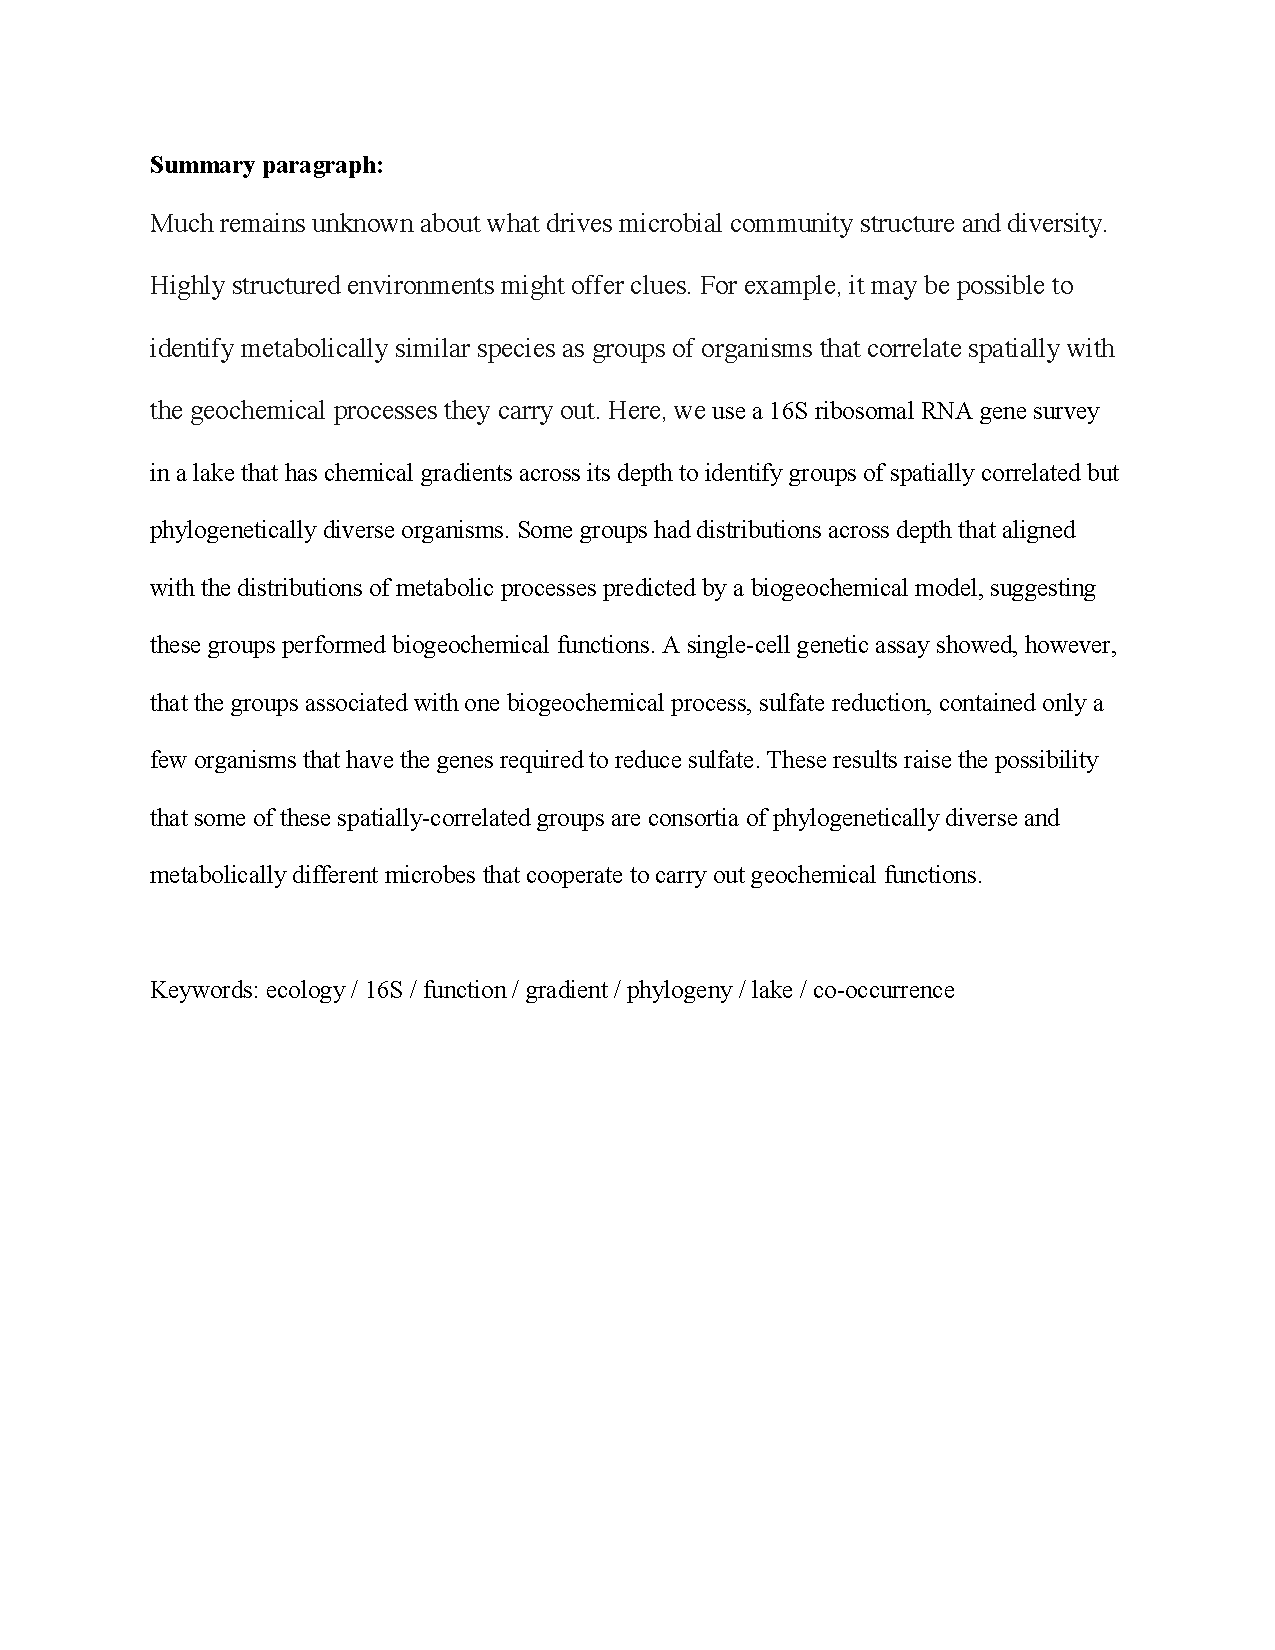
\includepdf[pages=-, pagecommand={\thispagestyle{plain}}]{lake/ms}

\begin{figure}[ht]
\centering
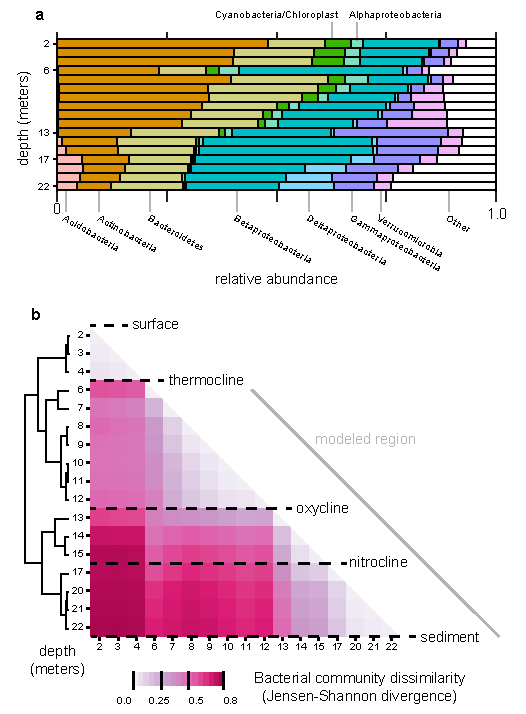
\includegraphics{lake/fig/fig1}
\caption*{{\bf Figure 1.} Bacterial survey of the lake identified communities
that vary with depth. {\bf a} The relative abundance of the seven most abundant phyla
at four representative depths. Proteobacteria is divided into the classes $\alpha$-,
$\beta$-, $\gamma$-, and $\delta$-Proteobacteria. ($\varepsilon$-Proteobacteria were 
not abundant [$< 0.5\%$ at
every depth] and are not shown.) {\bf b} Each square shows the dissimilarity between
bacterial communities at two depths (e.g., the lower-left square shows the
dissimilarity between the samples from the surface and from 22 meters depth).
Major features (dotted lines) of the lake are noted: the thermocline, where the
temperature gradient is steepest; the oxycline, where dissolved oxygen falls to
0.3 mg/L; the nitrocline, where nitrate concentration falls below detection;
and the sediment at the lake bottom. The biogeochemical model treats the region
below the thermocline (gray line).}
\end{figure}

\begin{figure}[ht]
\centering
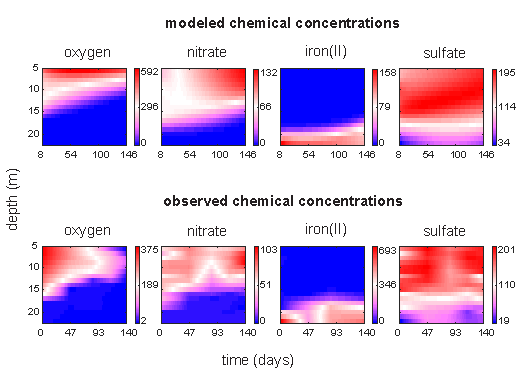
\includegraphics{lake/fig/fig2}
\caption*{{\bf Figure 2.} The model creates a dynamic picture of chemical
changes that occur in the lake through the lake's depth (vertical axis) across
time (horizontal). The model predicts changes in chemical species (top row;
colorbar scales are $\mu$M) which are consistent with the observed chemical
dynamics within the lake in 2013 (bottom row; colorbar scales are $\mu$M;
interpolated from five timepoints for oxygen, nitrate and sulfate and
interpolated from four time points for iron). The model was initiated from the
observed conditions in March 2013. Only a subset of chemical species included
in the model are shown.}
\end{figure}

\begin{figure}[ht]
\centering
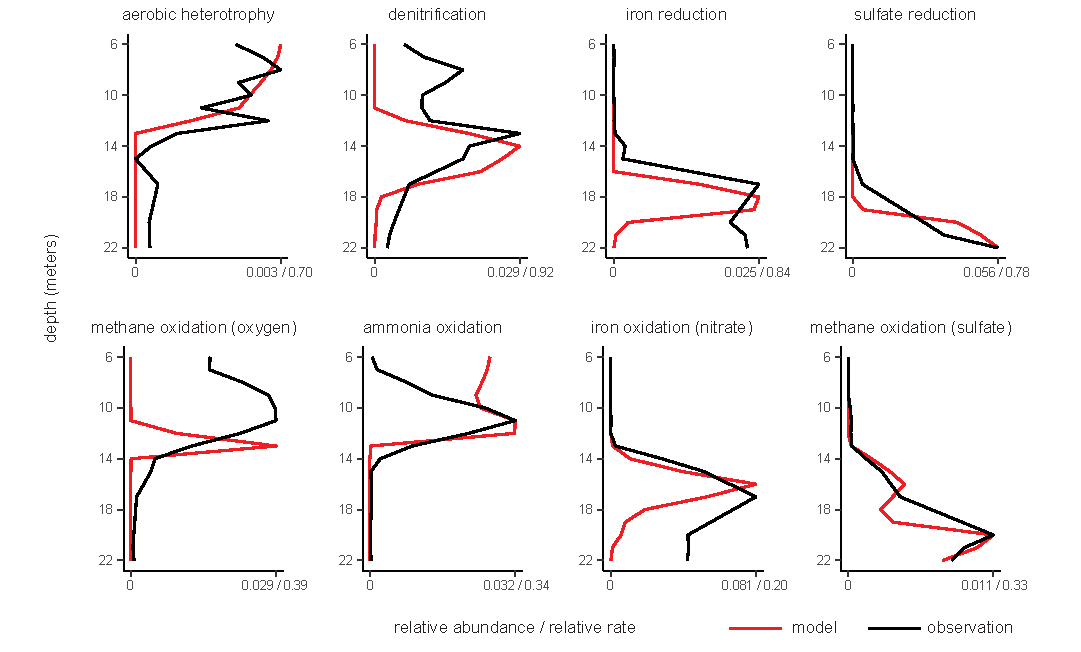
\includegraphics[width=\textwidth]{lake/fig/fig3}
\caption*{{\bf Figure 3.} Distribution of key populations (black lines,
relative abundance) from 2013 and their correspondence with modeled processes
(red lines, relative rate). Even though the two sets of lines represent
entirely different quantities (relative abundance of an organism vs. relative
prevalence of a metabolic process) their peaks and sometimes their spreads
roughly correspond, suggesting that the distribution of these organisms is
largely determined by the relative favorability of the modeled metabolic
processes within the lake.}
\end{figure}

\begin{figure}[ht]
\centering
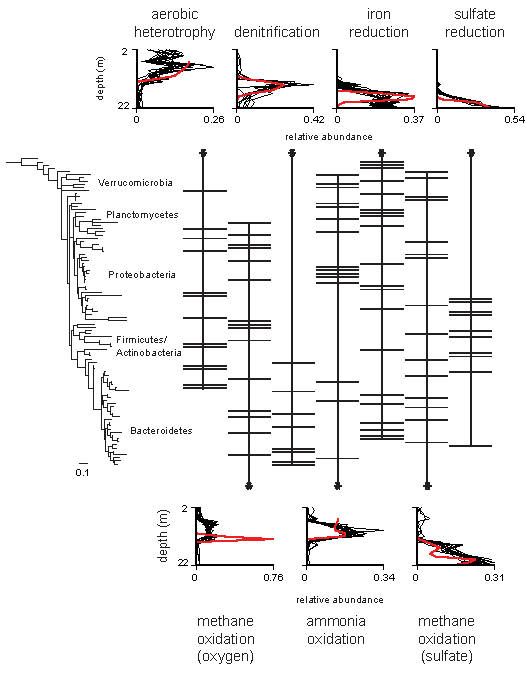
\includegraphics{lake/fig/fig4}
\caption*{{\bf Figure 4.} Operational ecological units (OEUs) are comprised of
phylogenetically diverse OTUs that largely align with modeled processes. The
phylogenetic tree (left; scale bar is substitutions per site) shows the
relationship between OTUs' representative 16S rRNA gene sequences in OEUs
containing key populations. Every OTU (on the rows) in the tree is a member of
one OEU (on the columns). Each bar indicates that the OTU in that row belongs
to the OEU represented by that column. Each inset shows the distributions
(black lines) with depth for OTUs in that OEU as well as the distribution (red
line) of a biogeochemical process (inset labels) predicted by the model. The
insets above and below the main figure correspond to the adjacent OEU columns
marked by asterisks. Modeled processes are only shown for the modeled region,
i.e., below 5 meters depth. OEUs were matched to the modeled processes as
described in the Methods.}
\end{figure}

\begin{figure}[ht]
\centering
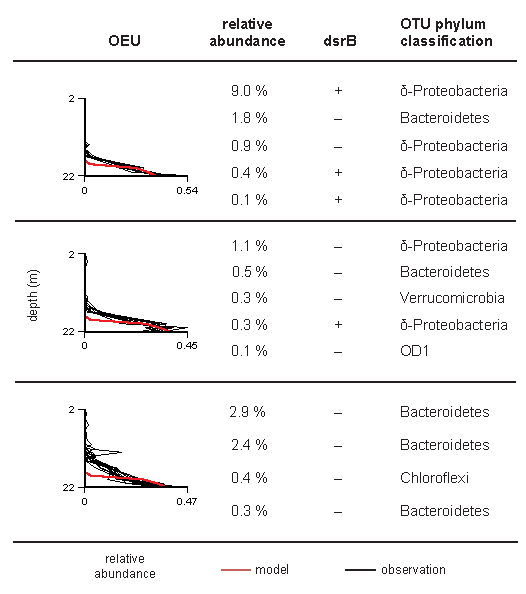
\includegraphics{lake/fig/fig5}
\caption*{{\bf Figure 5.} OEUs corresponding to sulfate reduction do not have
metabolically identical OTUs. The three OEUs with profiles corresponding to
sulfate reduction in the model are shown (the black lines are OTUs within each
OEU; the red lines are the relative rate of sulfate reduction predicted by the
model). The rows in each OEU correspond to each of that OEU's member OTUs. Of
these three OEUs, the single-cell assay determined that two OEUs contained
member OTUs that carry the diagnostic enzyme for sulfate reduction. The
relative abundance in the second column is percent of the control non-specific
16S-barcode fusion library corresponding to each OTU sequence. The third column
indicates whether a fusion product was identified in the \textit{dsrB}-16S gene fusion
library ($+$/$-$). The fourth column indicates phylum level classification for each
OTU, even if the OTU could be classified at a lower taxonomic rank.}
\end{figure}

%% This is an example first chapter.  You should put chapter/appendix that you
%% write into a separate file, and add a line \include{yourfilename} to
%% main.tex, where `yourfilename.tex' is the name of the chapter/appendix file.
%% You can process specific files by typing their names in at the 
%% \files=
%% prompt when you run the file main.tex through LaTeX.
\chapter{Designing fecal microbiota transplant trials that account for differences in donor stool efficacy}

The contents of this chapter were submitted with
Scott W. Olesen$^*$, Thomas Gurry$^*$ (these authors contributed equally), and Eric J. Alm as authors.

The supplementary information is in Appendix B.
The supplementary tables are at the end of the chapter.

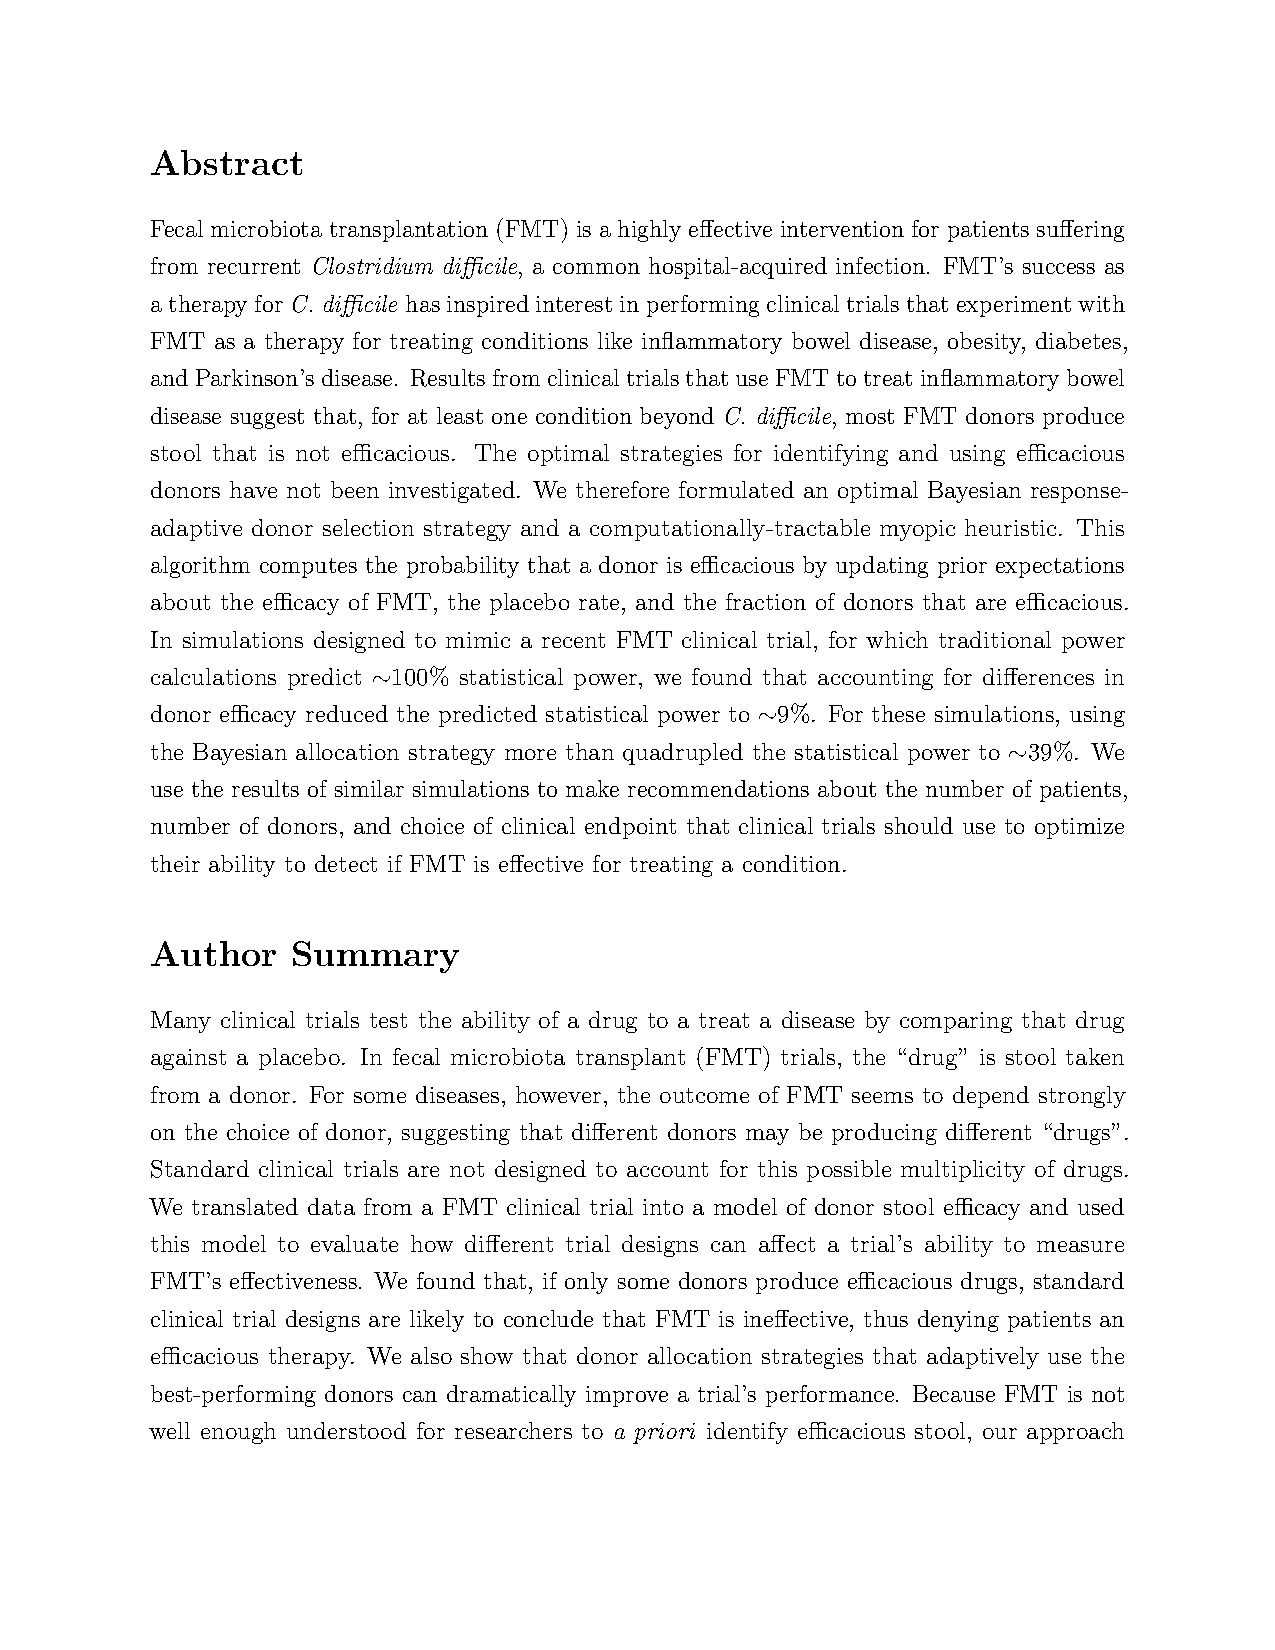
\includepdf[pages=-, pagecommand={\thispagestyle{plain}}, scale=0.95]{fmt/ms}

%% This is an example first chapter.  You should put chapter/appendix that you
%% write into a separate file, and add a line \include{yourfilename} to
%% main.tex, where `yourfilename.tex' is the name of the chapter/appendix file.
%% You can process specific files by typing their names in at the
%% \files=
%% prompt when you run the file main.tex through LaTeX.
\chapter{Discussion}

\section{Summary and limitations of reported work}
This thesis describes contributions to the interpretation of microbial
ecology sequence data and to the design of clinical trials. These contributions
each have limitations that restrict their validity and applicability.

In Chapter 2, I introduced \texttt{texmex}, a tool designed to quantify the dynamics of
microbial taxa in microbial ecology experiments that use amplicon sequence
data, use pre-tests, and have few or no replicates. I expect this approach
will be helpful when researchers want to analyze a pilot experiment, the
environmental inoculum is difficult to acquire, or the experimentation is
particularly onerous. Ideally, a researcher would perform many replicate
experiments and use that information for a rigorous statistical inference that
does not require any special consideration of the ecological structure of the
data in question, thus obviating the need for a technique like \texttt{texmex}.
Because the method is not statistical, however, it will never supplant
methods that are designed to determine whether two sets of measurements are
meaningfully different from a statistical standpoint.

In Chapter 3, I introduced the operational ecological unit (OEU) and
the inferred biomass interpretative framework to link taxonomic survey data, an
ecosystem-level metabolic model, and the results from a single-cell genetic
assay. The model itself is conceptual and intentionally simple; it therefore
lacks the ability to describe complicated features of the lake
ecosystem it models. For example, the model could never predict the
hypolimnetic oxygen minimum observed in the survey data. Operational
ecological units are essentially statistical and not necessarily functional,
so it is not straightforward to confirm or disprove their ``existence''. The
utility of the OEU concept could be evaluated by comparing an analysis of OEUs
with a large database of known ecological interactions. The inferred biomass
framework makes concrete, verifiable claims about microbial community function
that could be compared with metagenomic data and, ultimately, verified or
disproved by comparison with an exhaustive, \textit{in situ} survey of
ecosystem function. The results of the study are overall very suggestive, but
they are not experimentally verified and would require extensive co-culturing
or perturbative, \textit{in situ} metabolic experiments to validate.

In Chapter 4, I introduced a model of differences in donors' stool with
respect to its probability to cause patients to respond to treatment with fecal microbiota
transplant. The model makes concrete predictions about the utility of clinical
trial designs, but the structure of the model is based on a small amount of
clinical trial data and would require extensive clinical trial data to verify.
This study is in a catch-22: it aims to improve the probability of finding the
statistically-significant clinical trial data that would provide the only way to
assess the validity of the model.

\section{Potential extensions of reported work}
\subsection{Rank-abundance distributions and small data}
In a narrow sense, \texttt{texmex} is a software package that converts OTU tables
into tables of values related to the initial counts and provides convenience
functions for manipulating and selecting interesting OTUs based on those
transformed values. More broadly, that work makes two contributions that should
be helpful for future efforts to improve the interpretability of DNA sequence
data in microbial ecology.

First, I was surprised that I could find no studies that directly
examined or utilized the rank-abundance distribution of microbial ecology
sequence data. (I found only one paper that fit a rank-abundance distribution to
microbial ecology data~\cite{kembel_incorporating_2012}, and I describe what I
perceive as deficiencies in the logic of its application in Chapter 2.) I
believe that there are many applications that will emerge from using such
rank-abundance distributions, just as $z$-scores make normally-distributed data
more tractable for analysis. In particular, I expect that any attempt to
compare OTUs across samples could benefit from the kind of ``normalization''
that \texttt{texmex} does.
The standard statistical approach, in which an OTU's counts across samples are
modeled as variates of a single random variable, seems like a weak approach
compared to focusing on the ecological processes that cause the entire community
to assemble.

This sort of sample-wise approach should also be helpful for understanding some
of the more confusing aspects of microbiome data, particularly the zeros and
the effects of rarefaction.
It is becoming clearer that micro- and macroecology can share their methods~\cite{hughes_counting_2001},
so microbial ecologists should, in some cases, pay closer attention to the
methods and approaches used in traditional ecology.

Second, \texttt{texmex} starts from a very different place from many other
analytical methods: it assumes a paucity of data rather than an abundance.
As DNA sequencing has become cheaper, it is tempting to believe that microbial
ecology is now limited only by the cleverness of the algorithms used to generate
the data or the cleverness of the scientists who decide what questions to
investigate. In fact, sample acquisition is still, in many cases, a limiting
factor in microbial ecology, as has been my experience in the project described
in Chapter 2 (as well as in a separate project in coordination with the Department
of Energy).
If a study is not comfortably in the regime of
big data, I believe it is wiser to relegate yourself to the regime of small
data. Although you can ``do statistics'' with three samples, if you cannot
get twenty samples, it might be wiser to collect two and use a small-data
technique for the first experiment. As reviewers of the manuscript pointed
out, it is always better, \textit{ceteris paribus}, to have more replicates.
My point is that having more replicates always come at some cost, and the
added replicates might deliver a $p$-value without any additional scientific insight.

I was impressed that a recent paper studying oil degradation pathways in
samples collected from the Deepwater Horizon spill---and which used an impressive
combination of isotope labeling and metagenomic sequencing---identified similar organisms
as my algorithm did~\cite{dombrowski_reconstructing_2016}, showing the power
that small data and wise analytics can have.

There were extensions of this work that were outside the scope of this
thesis. Are there datasets that are sufficiently well-resolved to be able
to distinguish the rank-abundance distribution of microbial ecosystems?
Is that distribution the Poisson-lognormal distribution or something else? Is it different
for different ecosystems? What does that tell us, theoretically,
about the structure of those communities? Can we use rank-abundance models
to avoid the problems that compositional data present for analysis?
Can we use rank-abundance distributions to infer more rational models of
the behavior of taxa across samples? Relatedly, can we use rank-abundance
models and timeseries data to draw inferences about the dynamical behaviors
of individual taxa and entire bacterial communities? Can we better explain
the overdisperse and apparently noisy behavior of taxa through time?

\subsection{Modeling, consortia, and combinations of methodologies}
Like \texttt{texmex},
the methods used for the project described in Chapter 3 also aimed to extract the maximum amount of
insight from limited data. This project integrated the results from
multiple methods to yield a single, biologically-interpretable discovery.
This integration carries some lessons of its own.

First, models of microbial communities should aim for an optimum between complexity
and falsifiability. Because the data generated by DNA sequencing are so
massive and so complicated, it is tempting to make a complicated model
of their behavior. However, even if such a model were made and even if it
correctly recapitulated the system's behavior, are we better off for
having it? For example, the model reported in this project used abstract
categories (e.g., sulfate reduction) to describe microbes' behavior.
The identity of the microbes that seemed to belong in that abstract
category was determined separately, and it is the link between the
microbes' identity and the abstract behavior in the model that was useful.
If the model had perfectly described the behavior of every microbial
species, then we would have produced a system exactly as complicated
as the natural one, which would not advance our ability \emph{interpret}
the system.

Indeed, one of the strengths of the model presented in that work is that
it was \textit{a priori} unclear if it would even remotely recapitulate the lake's chemical
dynamics. If it did not, then it would be immediately clear that our mental
picture of the processes that shape the lake's behavior was largely
incomplete. Adding another process into the model (e.g., the interaction
between iron and sulfur) would hold the model and the associated data
to a much more stringent measure: it would require a great enough precision
in the data to be able to distinguish between the cases in which the
iron-sulfur interactions are included or not. Given the year-to-year
variability in this system, an ecosystem-wide model is not the appropriate
tool for making that discrimination. The simple fact that the model
worked at all---and that, if it had not worked, we would have learned
something too---is its major contribution. A model that is not interesting
if it fails is one that should not be considered interesting if it
succeeds.

There is probably great opportunity for modeling in microbial systems.
The model used in this project was based on a pre-next-generation-sequencing
model of microbes in a groundwater aquifer responding to pollutants,
which also highlights the fact that literature from before 1990 can
be full of interesting insights and thorny questions that we now have
the tools to explore more deeply.

For example, despite direct measurements of bacterial growth in
zebrafish~\cite{jemielita_spatial_2014} and a bacterium genetically
engineered to answer questions about the rate of division in the gut~\cite{myrhvold_distributed_2015},
I have not seen a model of division and colonization in the mammalian
gut that accounts for its directionality: how does the unidirectional transport
of vast quantities of microbes from the ``top'' to the ``bottom'' affect
the microbial composition in the gut? Are downstream populations
less diverse than upstream populations because every microbial species
present at the bottom must have once been near the top?

Second, this project makes an early, unrefined estimate of the prevalence
of microbial consortia in natural environments. Before nucleotide sequencing,
bacterial species were distinguished based on their appearances or tests
of their metabolisms. This process was finicky and low throughput, so we
had vastly underestimated the diversity of microbes. I believe we are on
the cusp of a similar revelation about microbial consortia. I expect that
theoretical arguments would show that a large number of cooperative species
should be expected, and this contrasts against the very small number of
consortia that are known and studied. The possibility that there are
large numbers of consortia in many ecosystems is probably the most
scientifically interesting and important result in this thesis.

Third, this project shows the potential that combinations of methods
can play in understanding microbial systems. Surveys on their own
do little to address microbial function; models on their own
can seem like intellectual playgrounds unconnected to reality; high-throughput
screens on their own can generate large amounts of data with small amounts
of insight. In particular, I expect that combinations of models, surveys,
and metabolite measurements will provide interesting and useful
information about the interactions between microbial species (and hosts if
they have them).

\subsection{Decision-making in microbiome science}
The third project in this thesis is an outlier: it describes a
simple model---like Chapter 3 does---but it uses the model for
an entirely different purpose. Rather than developing information
about the possible behavior of a system, it uses a model and data to
make a decision in face of a question. (This distinction is reminiscent
of the difference in interpretations of the $p$-value~\cite{goodman_toward_1999} between Fisher,
who originally formulated it as a method to discern truth~\cite{fisher_statistical_1973}
and Neyman and Pearson, who saw it as a way to decide actions~\cite{neyman_problem_1933}.)
I will venture to say that most models in the world are, like this one,
operational models: they are designed to integrate data to inform a 
decision.

DNA sequencing is already being used in medicine to, for example,
diagnose infections, and there is hope that more sophisticated,
rapid, point-of-care diagnostics will be useful to, say, use information
about the genetics of the pathogen to decide
which antibiotic to administer to a patient.
However, the role of modeling in decision science
for microbiome science, as such, remains unclear. In what cases could
a large collection of information about the microbes inhabiting a
person's gut be useful for making a decision? What decision would
be made?

There are some appealing answers. Measurements of the microbiome
could be used to diagnose a disease that is otherwise difficult or
invasive to diagnose \cite{papa-noninvasive-2012}, to quantify the
risk that a patient will develop a disease, or to help stratify
patients based on the probability that they will respond to certain
drugs \cite{koeth-intestinal-2013,sivan-commensal-2015,vetizou-anticancer-2015}.
I expect a ``middle'' way will also be profitable. A model that
combines a simple treatment of a system (e.g., as in Chapter 4,
each donor is considered efficacious or not) and a more complex one
(e.g., it is asserted that the presence or absence of some microbial
taxon in the donor determines the probability of patient response)
could recommend decisions that are nearly optimal with respect to
the simple, operational model while deriving greater benefit for
the more complex, mechanistic model. This operational half of
the approach might get complex hypothesis-testing into the clinic,
since the simple half of the algorithm could be relied upon to
make sensible decisions even if it became clear that the complex,
mechanistic model was completely incorrect.

In general, I caution microbiome scientists against interpreting too
much from 16S sequencing data. The fact that DNA sequencing is a
less-biased way to enumerate communities than traditional 
culture-based methodologies may have reduced the emphasis on the
problems that DNA sequencing presents: the microbiome appears to
be a dynamic, noisy system; extraction and preparation methodologies
greatly affect the output signal; different bioinformatic techniques
can lead to different scientific conclusions; and proper methods
of statistical analysis for these data are still under debate.
Targeted questions with large sample sizes and perturbative
techniques are the best avenue for conclusions; small experiments
with decidedly exploratory analytical methods are the best
avenue for developing avenues for fuller investigation.

\epigraph{{\selectlanguage{polutonikogreek}κτῆμά τε ἐς αἰεὶ μᾶλλον
ἢ ἀγώνισμα ἐς τὸ παραχρῆμα ἀκούειν ξύγκειται.}}{Thucydides, \textit{History}, 1.22.4}

\begin{singlespace}
\bibliography{main}
\bibliographystyle{unsrt}
\end{singlespace}

\appendix
\chapter{Supplementary Information for Chapter 3}

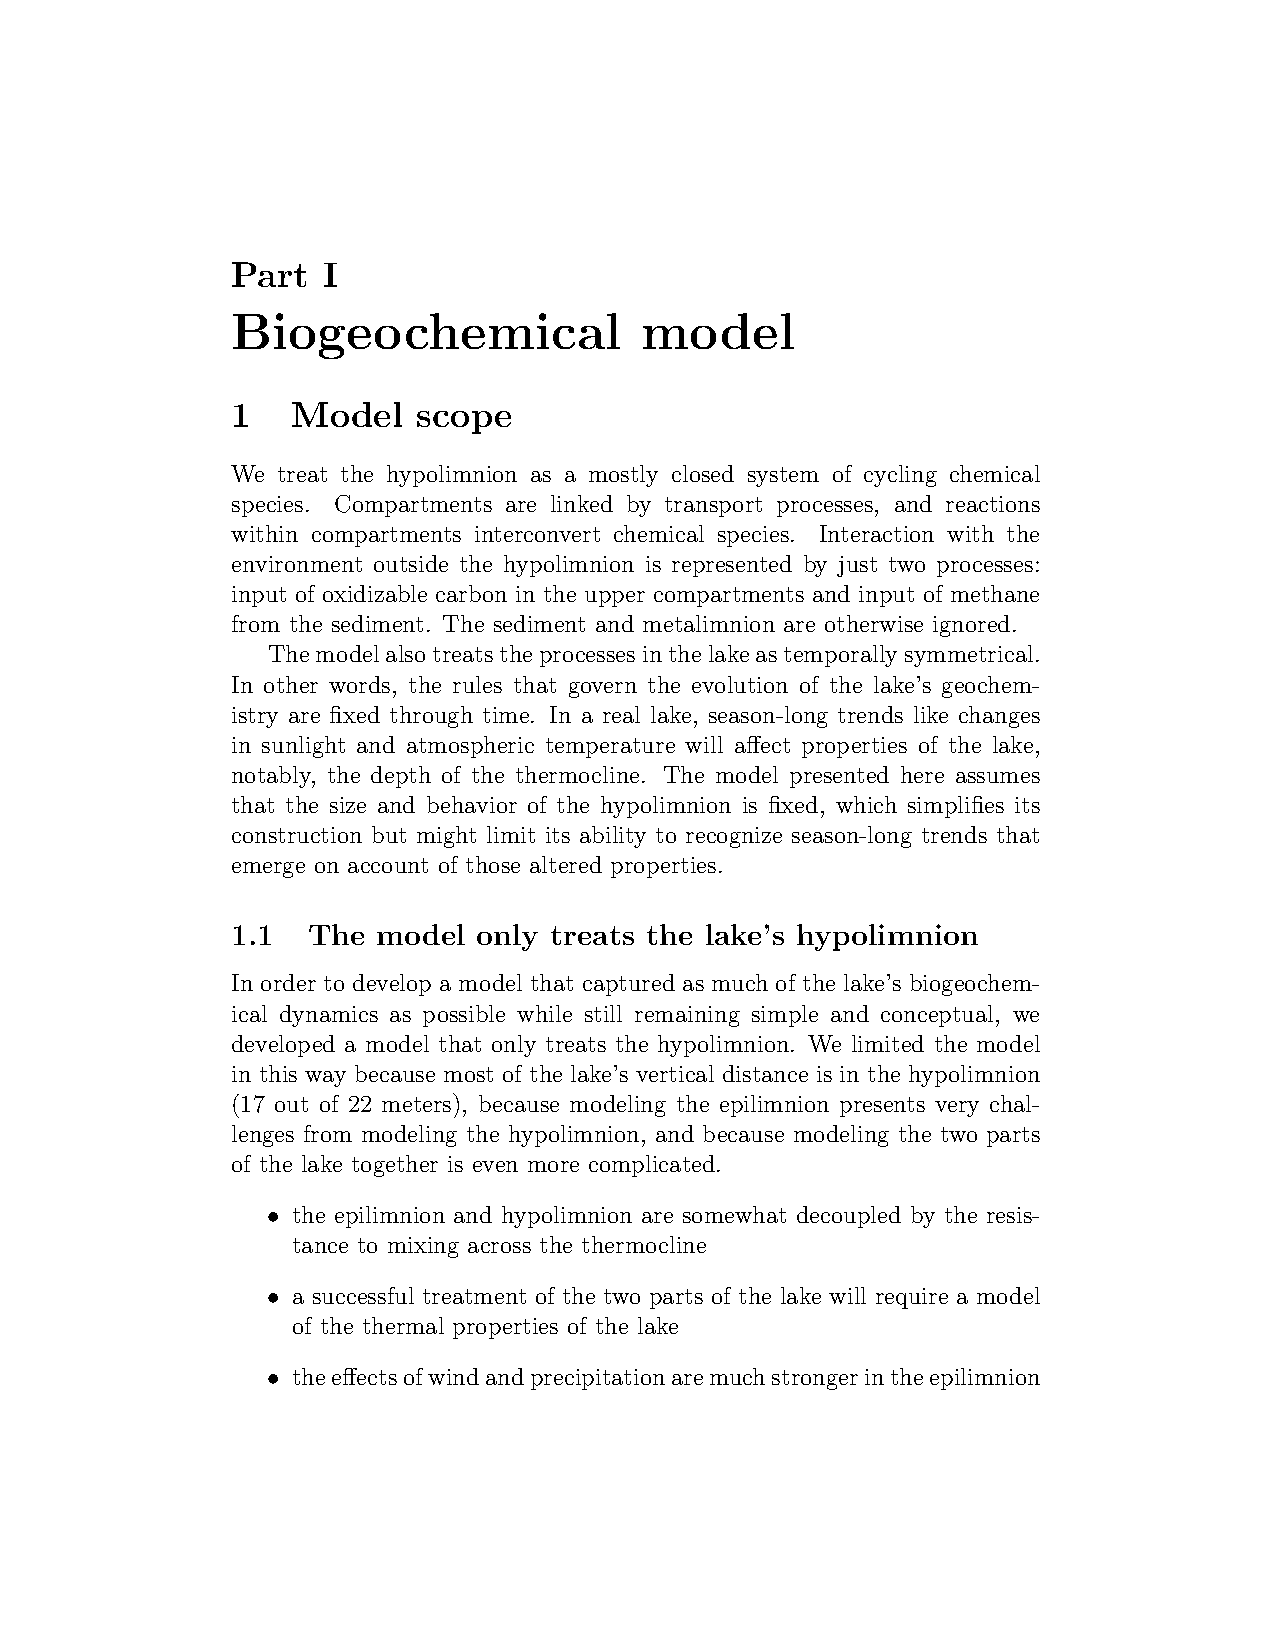
\includepdf[pages=-, pagecommand={\thispagestyle{plain}}]{lake/si}

\chapter{Supplementary Information for Chapter 4}

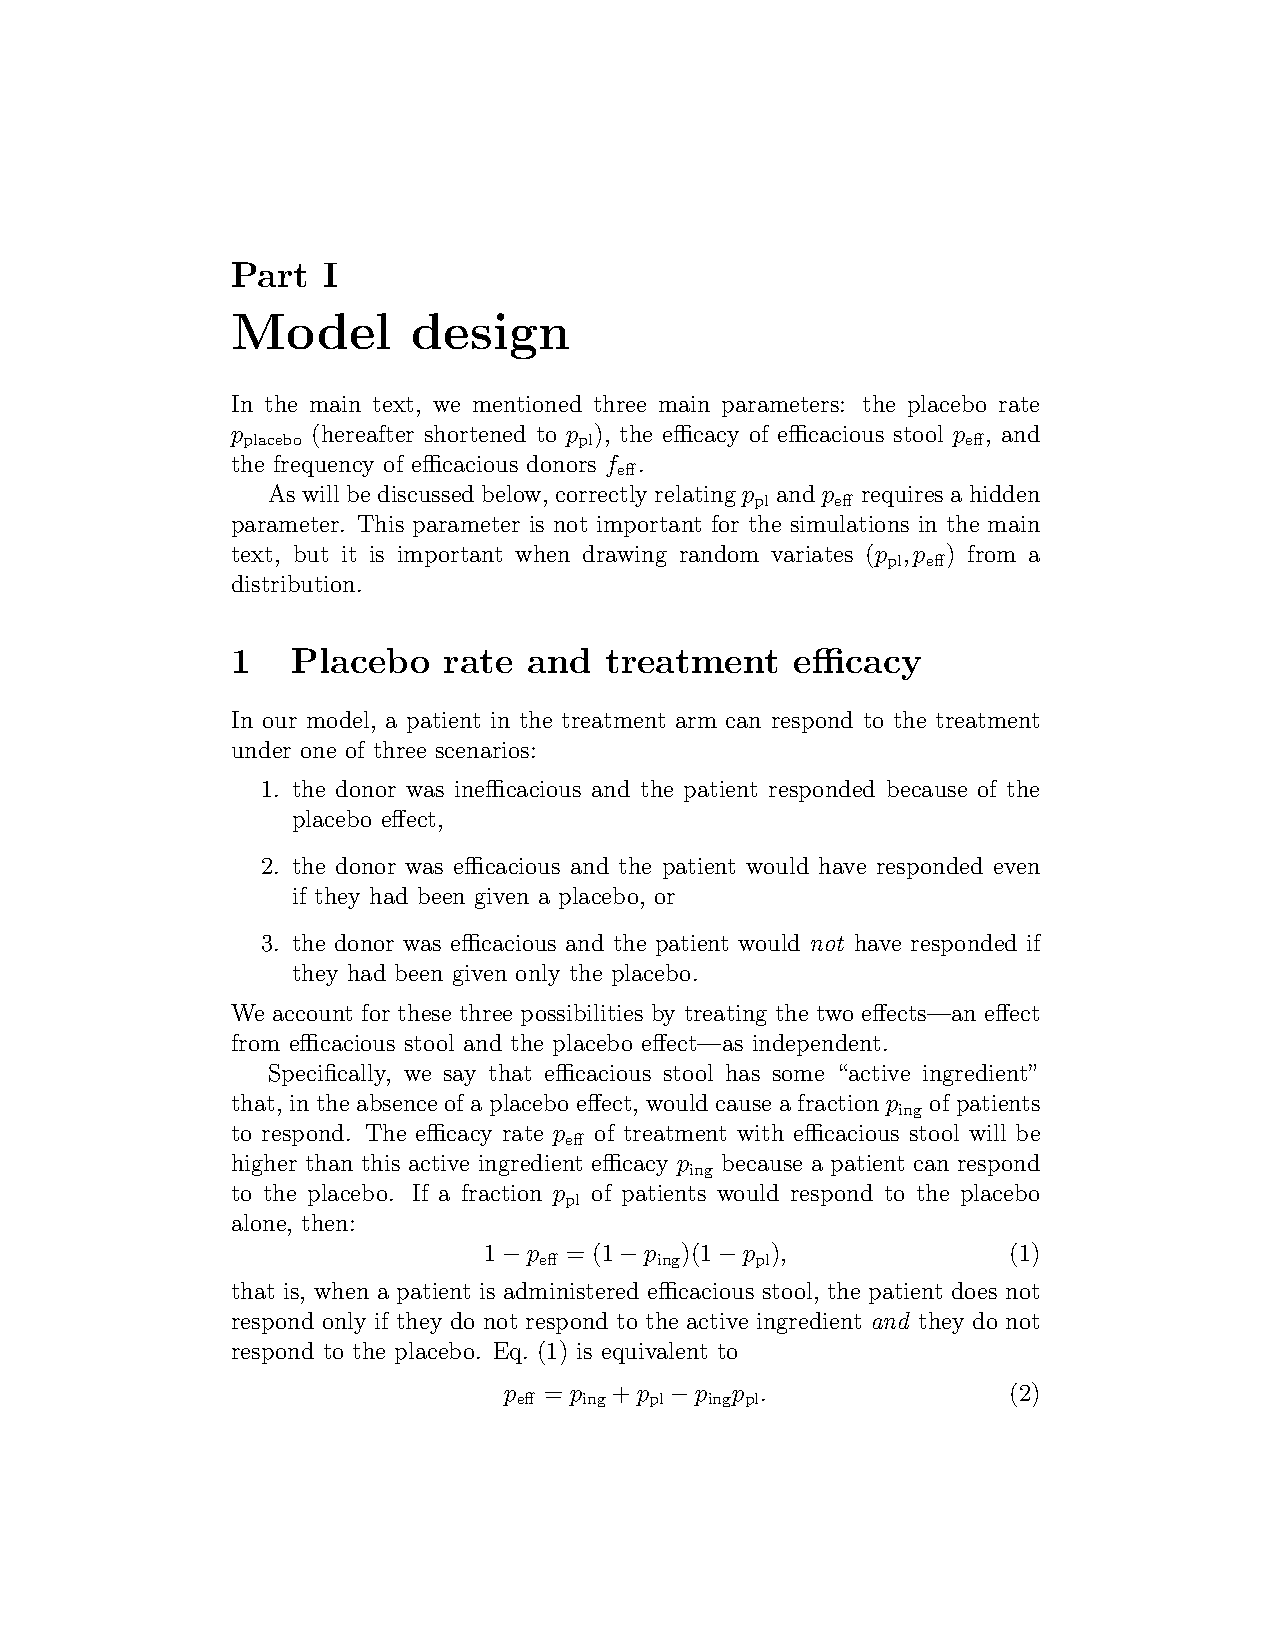
\includepdf[pages=-, pagecommand={\thispagestyle{plain}}]{fmt/si}

% Include the biblio file if you want to have a single, monolithic list of references
% at the end of the thesis. If you do not include the biblio file, you'll have to put
% bibliographies at the end of each chapter.
%%% This defines the bibliography file (main.bib) and the bibliography style.
%% If you want to create a bibliography file by hand, change the contents of
%% this file to a `thebibliography' environment.  For more information 
%% see section 4.3 of the LaTeX manual.
\begin{singlespace}
\bibliography{main}
\bibliographystyle{plain}
\end{singlespace}


\end{document}
